


\documentclass[10pt]{NSP1}
\usepackage{url,floatflt}
\usepackage{helvet,times}
\usepackage{psfig,graphics}
\usepackage{mathptmx,amsmath,amssymb,bm}
\usepackage{float}
\usepackage[bf,hypcap]{caption}

\usepackage[dvipsnames,table,xcdraw]{xcolor}

\tolerance=1
\emergencystretch=\maxdimen
\hyphenpenalty=10000
\hbadness=10000

\topmargin=0.00cm

\def\sm{\smallskip}
\def\no{\noindent}

\def\firstpage{1}
\setcounter{page}{\firstpage}
\def\thevol{1}
\def\thenumber{1}
\def\theyear{2015}


\begin{document}

\titlefigurecaption{{\large \bf \rm Progress in Fractional Differentiation
and Applications}\\ {\it\small An International Journal}}

\title{Local Fractional Variational Iteration Algorithms for the
Parabolic Fokker-Planck Equation Defined on Cantor Sets}

\author{Dumitru Baleanu{$^{1,2}$}, Hari M. Srivastava{$^3$} and Xiao-Jun Yang{$^{4,*}$}}
\institute{Department of Mathematics and Computer Sciences, Faculty of Arts and
Sciences, Cankaya University, TR-06530 Ankara, Turkey\and
Institute of Space Science, R-077125 M\u{a}gurle-Bucharest, Romania \and
Department of Mathematics and Statistics, University of Victoria,
Victoria, British Columbia V8W 3R4, Canada\and Department of
Mathematics and Mechanics, China University of Mining
and Technology, Xuzhou, Jiangsu 221008, People's Republic of China}

\titlerunning{Local Fractional Variational Iteration Algorithms ...}
\authorrunning{D. Baleanu et al. }


\mail{dyangxiaojun@163.com}

\received{2 Sep. 2014}
\revised{18 Oct. 2014}
\accepted{20 Nov. 2014}
\published{1 Jan. 2015}

\abstracttext{In this article, we apply the local fractional variational iteration algorithms
for solving the parabolic
Fokker-Planck equation which is defined on Cantor sets. It is shown by
comparing with the three LFVIAs that the LFVIA-II is the easiest to obtain the
non-differentiable solutions for linear local fractional partial
differential equations. Several other related recent works dealing
with local fractional derivative operators on Cantor sets are also indicated.}

\keywords{Approximate solution, parabolic Fokker-Planck equation, local fractional
derivative operators, Cantor sets.\\[2mm]
\textbf{2010 Mathematics Subject Classification}.  Primary 26A33, 35A20; Secondary 33B15.}

\maketitle

\section{\; Introduction, Motivation and Preliminaries}

Fractional calculus \cite{1,2,3,4,5,6,7,8,9} has found successful applications in science and
engineering, such as fractional-order signals, physics, bioengineering, and
dynamics of particles. As an important fractional-order PDEs arising
in mathematical physics, the space-and time-fractional Fokker-Planck
equation was first derived from the generalised master equation \cite {10} with
the time-fractional derivative and after that it ws developed in \cite {11}. Based
on it, Barkai \cite {12} successfully found the solutions of the continuous time
random walk, whistle Odibat and Momani \cite {13} suggested VIM and ADM to solve
it. Meanwhile, Den presented the FEM to obtain the numerical solution \cite {14}.
A new version of the time-fractional FP equation was suggested by using
dynamical systems of FBM \cite {15} and the fractal time evolution with a critical
exponent \cite {16}. Another version of the space-fractional FP equation from the
fractional Liouville equation via fractional-power systems \cite {17,18} and the
fractional-order governing equation of L\'{e}vy motion \cite {19} was reported.
Based on this, the upwind difference method was considered by Liu \cite {20} to
deal with it. Meanwhile, the finite difference method was proposed by Chen
et al. \cite {21} to solve it.

The various versions of local fractional calculus theory
\cite{22,23,24,25,26,27,28,29,30,31,32,33} were
considered to describe the non-differentiable problems from local fractional
PDEs in physics and science due to the surface and structure of materials,
which are so-called fractals \cite {34}. Local fractional VIM \cite {35,36} was one of
usual methods for finding non-differentiable solutions for the local
fractional PDEs. The FP equation defined on Cantor sets was presented as
follows (see \cite{37,38}):
\begin{equation}
\label{eq1}
\frac{\partial ^\alpha }{\partial \zeta ^\alpha }\varphi \left( {\zeta ,\eta
} \right)=-\frac{\partial ^\alpha }{\partial \eta ^\alpha }\varphi \left(
{\zeta ,\eta } \right)+\frac{\partial ^{2\alpha }}{\partial \eta ^{2\alpha
}}\varphi \left( {\zeta ,\eta } \right).
\end{equation}
The parabolic equation defined on Cantor sets can be presented as follows:
\begin{equation}
\label{eq2}
\frac{\partial ^\alpha }{\partial \zeta ^\alpha }\varphi \left( {\zeta ,\eta
} \right)=\chi \left( {\zeta ,\eta } \right)\frac{\partial ^\alpha
}{\partial \eta ^\alpha }\varphi \left( {\zeta ,\eta } \right)+\kappa \left(
{\zeta ,\eta } \right)\frac{\partial ^{2\alpha }}{\partial \eta ^{2\alpha
}}\varphi \left( {\zeta ,\eta } \right),
\end{equation}
where $\chi \left( {\zeta ,\eta } \right)$ and $\kappa \left( {\zeta ,\eta }
\right)$ are parameters.

The goal of this article is to suggest the local fractional variational
iteration algorithms (LFVIAs) \cite {39,40} to the parabolic equation defined
above on Cantor set.

This article is organized as follows.
In Section 2, we review the local fractional calculus theory. In Section 3,
the local fractional variational iteration algorithms are analyzed. In
Section 4, the non-differentiable solution for the parabolic Fokker-Planck
equation defined on Cantor sets is obtained. Finally, the conclusions are
provided in Section 5.

\section{\; Local Fractional Calculus Theory}
In this section, we first introduce the concepts and notations of the theory
of the local fractional calculus. To begin with, we recall the result for
the local fractional continuity.

Let $\wp$ be a subset of the real line and be a fractal. If $g:\left( {\wp
,\rho } \right)\to \left( {\Xi ,\rho } \right)$ is a bi-Lipschitz mapping,
then (for constants $\mu ,\eta >0$ and $\wp \subset \mathbb{R} $) we have
\begin{equation}
\label{eq3}
\mu ^sH^s\left( \wp \right)\leqq H^s\big( {g\left( \wp \right)}\big)\leqq
\eta ^sH^s\left( \wp \right)
\end{equation}
such that, for all $\zeta _1 ,\zeta _2 \in \wp $,
\begin{equation}
\label{eq4}
\mu ^\alpha \left| {\zeta _1 -\zeta _2 } \right|^\alpha \leqq \left| {g\left(
{\zeta _1 } \right)-g\left( {\zeta _2 } \right)} \right|\leqq \eta ^\alpha
\left| {\zeta _1 -\zeta _2 } \right|^\alpha .
\end{equation}
Following (\ref{eq4}), we have
\begin{equation}
\label{eq5}
\left| {g\left( {\zeta _1 } \right)-g\left( {\zeta _2 } \right)} \right|\leqq
\eta ^\alpha \left| {\zeta _1 -\zeta _2 } \right|^\alpha,
\end{equation}
which yields
\begin{equation}
\label{eq6}
\left| {g\left( {\zeta _1 } \right)-g\left( {\zeta _2 } \right)} \right|\le
\varepsilon ^\alpha,
\end{equation}
where $\left| {\zeta _2 -\zeta _1 } \right|<\kappa $, $\varepsilon ,\kappa
>0$, and $H^\alpha _{ }$ is an $\alpha$-dimensional Hausdorff measure.

Using (\ref{eq6}), one leads to the following relation:
\begin{equation}
\label{eq7}
\mathop {\lim }\limits_{\zeta \to \zeta _1 } g\left( \zeta \right)=g\left(
{\zeta _1 } \right),
\end{equation}
which exhibits the fact that $g\left( \zeta \right)_{ }$ is a so-called local
fractional continuous function at $\zeta =\zeta _1 $.

We write
\begin{equation}
\label{eq8}
g\left( \zeta \right)\in C_\alpha \left( {\sigma ,\upsilon } \right),
\end{equation}
if $g\left( \zeta \right)_{ }$is only a local fractional continuous
function on the interval $\left( {\sigma ,\upsilon } \right)$.

In order to make very fine distinction from the classical continuous function theory,
we consider the new form (\ref{eq6}) as the local fractional continuous condition.
We notice that the constant is the special function because it belongs to
either Lipschitz or bi-Lipschitz.

The $\alpha$-dimensional Hausdorff measure given by (see \cite{41})
\begin{equation}
\label{eq9}
H^\alpha \left( {\wp \cap \left( {\sigma ,\upsilon } \right)} \right)=\left(
{\upsilon -\sigma } \right)^\alpha ,
\end{equation}
shows that $\alpha \mbox{ }\left( {0<\alpha <1} \right)$ is a fractal
dimension value, and it is the graph of Cantor function presented in \cite {42}
from $\sigma =0_{ }$ to $\upsilon =1$. Namely, it is directly deduced from
fractal geometry.

There also are several other useful functions as follows \cite {41}:
\begin{equation}
\label{eq10}
E_\alpha \left( {\zeta ^\alpha } \right)=\sum\limits_{i=0}^\infty
{\frac{\zeta ^{i\alpha }}{\Gamma \left( {1+i\alpha } \right)}} ,
\end{equation}
\begin{equation}
\label{eq11}
\sin _\alpha \zeta ^\alpha =\sum\limits_{i=0}^\infty {\frac{\left( {-1}
\right)^i\zeta ^{(2i+1)\alpha }}{\Gamma \left[ {1+\left( {2i+1}
\right)\alpha } \right]}}
\end{equation}
and
\begin{equation}
\label{eq12}
\cos _\alpha \zeta ^\alpha =\sum\limits_{i=0}^\infty {\frac{\left( {-1}
\right)^i\zeta ^{2\alpha i}}{\Gamma \left( {1+2\alpha i} \right)}} .
\end{equation}

For $0<\alpha <1$ and $g\left( \zeta \right)\in C_\alpha \left( {\sigma
,\upsilon } \right)$, we define the local fractional derivative of $g\left(
\zeta \right)$ of order $\alpha$ as follows (see \cite {22,23,35,36,37,38,39,40,41}):
\begin{equation}
\label{eq13}
g^{\left( \alpha \right)}\left( {\zeta _0 } \right)=\frac{d^\alpha g\left(
\zeta \right)}{d\zeta ^\alpha }\bigg|_{\zeta =\zeta_0}=\mathop
{\lim }\limits_{\zeta \to \zeta _0 } \frac{\Delta ^\alpha \big( {g\left(
\zeta \right)-g\left( {\zeta _0 } \right)} \big)}{\left( {\zeta -\zeta _0
} \right)^\alpha },
\end{equation}
where
$$\Delta ^\alpha \big( {g\left( \zeta \right)-g\left( {\zeta _0 }
\right)} \big)\cong \Gamma \left( {1+\alpha } \right)\Delta \big(
{g\left(\zeta \right)-g\left({\zeta_0} \right)} \big).$$

Let $0<\alpha <1$, $g\left( \zeta \right)\in C_\alpha \left( {\sigma
,\upsilon } \right)$, $_{ }\Delta s_j =s_{j+1} -s_j $,
$\Delta s=\max
\left\{ {\Delta s_1 ,\Delta s_2 ,\Delta s_j ,\cdots} \right\}_{ }$
and $\left[{s_j ,s_{j+1} } \right]$ $(j=0,\cdots,N-1)$ (with $s_0 =\sigma$
and $s_N =\upsilon$) be a
partition of the interval $\left( {\sigma ,\upsilon } \right)$. Define the
local fractional integral of $g\left( \zeta \right)$ of $\alpha $ order
\cite{22,23,35,36,37,38,39,40,41}
\begin{align}
\label{eq14}
{ }_\sigma I_\upsilon ^{\left( \alpha \right)}g\left( s
\right)&=\frac{1}{\Gamma \left( {1+\alpha } \right)}\int_\sigma ^\upsilon
{g\left( s \right)\left( {ds} \right)^\alpha }\notag\\
& =\frac{1}{\Gamma \left(
{1+\alpha } \right)}\mathop {\lim }\limits_{\Delta s\to 0}
\sum\limits_{j=0}^{j=N-1} {f\left( {s_j } \right)} \left( {\Delta s_j }
\right)^\alpha .
\end{align}
In view of (\ref{eq14}), we have the following relations:

\begin{equation}
{ }_\sigma I_\upsilon ^{\left( \alpha \right)}g\left( s \right)=0 \qquad (\sigma
=\upsilon)
\end{equation}
and
\begin{equation}
{ }_\sigma I_\upsilon ^{\left( \alpha \right)}g\left( s
\right)=-\;{ }_\upsilon I_\sigma ^{\left( \alpha \right)}g\left( s \right)\qquad
(\sigma <\upsilon).
\end{equation}

Basic formulas for the local fractional derivatives (LFDs) and the local
fractional integrals (LFIs) of the functions are listed in Table 1.\\

\begin{center}
\textbf{Table 1. List of local fractional derivatives and integrals of some
functions}
\end{center}

\begin{table}[htbp]
\begin{center}
\begin{tabular}{|p{180pt}|p{158pt}|}
\hline
LFDs&
LFIs \\
\hline
$\frac{d^\alpha }{d\zeta ^\alpha }g\left( \zeta \right)=0,$
\par where
$_{ }g\left( \zeta \right)_{ }$ is a given differentiable function &
${ }_0I_\zeta ^{\left( \alpha \right)}g\left( \zeta \right)$ does not exist
\par where $g\left( \zeta \right)_{ }$ is a given differentiable function \\
\hline
$\frac{d^\alpha }{d\zeta ^\alpha }E_\alpha \left( {\zeta ^\alpha } \right)
=E_\alpha \left( {\zeta ^\alpha } \right)$ &
${ }_0I_\zeta ^{\left( \alpha \right)}E_\alpha \left( {\zeta ^\alpha }
\right)=E_\alpha \left( {\zeta ^\alpha } \right)-1$ \\
\hline
$\frac{d^\alpha }{d\zeta ^\alpha }\left[ {\frac{\zeta ^\alpha }
{\Gamma \left( {1+2\alpha } \right)}} \right]=\frac{\zeta ^{2\alpha }}
{\Gamma \left( {1+\alpha } \right)}$ &
${ }_0I_\zeta ^{\left( \alpha \right)}\frac{\zeta ^\alpha }{\Gamma \left( {1+\alpha } \right)}
=\frac{\zeta ^{2\alpha }}{\Gamma \left( {1+2\alpha } \right)}$ \\
\hline
$\frac{d^\alpha}{d\zeta ^\alpha }\; \cos _\alpha \left( {\zeta ^\alpha } \right)
=-\sin _\alpha \left( {\zeta ^\alpha } \right)$ &
${ }_0I_\zeta ^{\left( \alpha \right)}\sin _\alpha \left( {\zeta ^\alpha }
\right)=1-\cos _\alpha \left( {\zeta ^\alpha } \right)$ \\
\hline
$\frac{d^\alpha}{d\zeta ^\alpha}\;
\sin _\alpha \left( {\zeta ^\alpha } \right)
=\cos _\alpha \left( {\zeta ^\alpha } \right)$ &
${ }_0I_\zeta ^{\left( \alpha \right)}\cos _\alpha \left( {\zeta ^\alpha }
\right)=\sin _\alpha \left( {\zeta ^\alpha } \right)$ \\
\hline
\end{tabular}
\label{tab1}
\end{center}
\end{table}

In Table 1, $g\left( \zeta \right)_{ }$ is a given differentiable function.
For more details of the fractional calculus and the local fractional calculus theory,
see \cite {22,23,35,36,37,38,39,40,41,42,43,44,45}.\\

\vskip 2mm

\section{\; The Local Fractional Variational Iteration Algorithms}

Let $\varphi ^{\left( \alpha \right)}\left( \zeta \right)$ take on the local
fractional differential operator and $\sigma \leqq x\leqq \upsilon $. In view of
a local fractional variational principle (see, for example, \cite {23,43}),
the local fractional function reads as follows:
\begin{equation}
\label{eq15}
\Pi \left( \varphi \right)={ }_\sigma I_\upsilon ^{\left( \alpha
\right)}g\left( {\zeta ,\varphi \left( \zeta \right),\varphi ^{\left( \alpha
\right)}\left( \zeta \right)} \right).
\end{equation}
The stationary condition of Eq. (\ref{eq15}) is given by
\begin{equation}
\label{eq16}
\frac{\partial g}{\partial \phi }-\frac{d^\alpha }{d\zeta ^\alpha }\left(
{\frac{\partial g}{\partial \phi ^{\left( \alpha \right)}}} \right)=0.
\end{equation}
Let $L_\alpha $ and $N_\alpha $be linear and nonlinear local fractional
operators respectively. A correction local fractional functional can be
structured as follows (see \cite {39,40}):
\begin{equation}
\label{eq17}
\varphi _{n+1} \left( \zeta \right)=\varphi _n \left( \zeta \right)+{
}_{\zeta _0 }I_\zeta ^{\left( \alpha \right)}\left\{ {\vartheta \left[
{L_\alpha \varphi _n \left( \tau \right)+N_\alpha \widetilde{\varphi }_n
\left( \tau \right)} \right]} \right\},
\end{equation}
where a general local fractional differential equation is presented as follows:
\begin{equation}
\label{eq18}
L_\alpha \varphi +N_\alpha \varphi =0,
\end{equation}
with a restricted local fractional variation $\widetilde{\varphi }_n $ and a
fractal Lagrange multiplier $\vartheta $, which is given by (\ref{eq16}).
After completing the identification of the fractional Lagrange multiplier of
(\ref{eq16}), the LFVIAs of three types have the following forms:
The LFVIA-I:
\begin{equation}
\label{eq19}
\varphi _{n+1} \left( \zeta \right)=\varphi _n \left( \zeta \right)+{
}_{\zeta _0 }I_\zeta ^{\left( \alpha \right)}\left\{ {\vartheta \left[
{L_\alpha \varphi _n \left( \tau \right)+N_\alpha \varphi _n \left( \tau
\right)} \right]} \right\}.
\end{equation}
The LFVIA-II:
\begin{equation}
\label{eq20}
\varphi _{n+1} \left( \zeta \right)=\varphi _0 \left( \zeta \right)+{
}_{\zeta _0 }I_\zeta ^{\left( \alpha \right)}\left\{ {\vartheta N_\alpha
\varphi _n \left( \tau \right)} \right\}.
\end{equation}
The LFVIA-III:
\begin{equation}
\label{eq21}
\varphi _{n+1} \left( \zeta \right)=\varphi _n \left( \zeta \right)+{
}_{\zeta _0 }I_\zeta ^{\left( \alpha \right)}\left\{ {\vartheta \left[
{N_\alpha \varphi _n \left( \tau \right)-N_\alpha \varphi _{n-1} \left( \tau
\right)} \right]} \right\}.
\end{equation}
Making use of the LFVIAs, the non-differentiable solution of (\ref{eq18}) reads as
follows:
\begin{equation}
\label{eq22}
\varphi =\mathop {\lim }\limits_{n\to \infty } \varphi _n .
\end{equation}
The present method is also utilized to  discuss the wave phenomena \cite{44,45}.\\

\vskip 2mm

\section{\; Non-Differentiable Solution}

Let $$\chi \left( {\zeta ,\eta } \right)=-\frac{2\zeta ^\alpha }{\Gamma
\left( {1+\alpha } \right)}\qquad \text{and} \qquad \kappa \left( {\zeta ,\eta }
\right)=\frac{3\zeta ^{2\alpha }}{\Gamma \left( {1+2\alpha } \right)}.$$ Then
the parabolic FK equation defined on Cantor sets with local fractional
derivative is given as follows:
\begin{equation}
\label{eq23}
\frac{\partial ^\alpha }{\partial \zeta ^\alpha }\varphi \left( {\zeta ,\eta
} \right)=-\frac{2\zeta ^\alpha }{\Gamma \left( {1+\alpha }
\right)}\frac{\partial ^\alpha }{\partial \eta ^\alpha }\varphi \left(
{\zeta ,\eta } \right)+\frac{3\zeta ^{2\alpha }}{\Gamma \left( {1+2\alpha }
\right)}\frac{\partial ^{2\alpha }}{\partial \eta ^{2\alpha }}\varphi \left(
{\zeta ,\eta } \right),
\end{equation}
and the initial condition is given by
\begin{equation}
\label{eq24}
\varphi \left( {0,\eta } \right)=\frac{\eta ^\alpha }{\Gamma \left(
{1+\alpha } \right)}.
\end{equation}
A correction local fractional functional can be structured as follows:
\begin{align}
\label{eq25}
&\varphi _{n+1} \left( {\zeta ,\eta } \right)
=\varphi _n \left( {\zeta ,\eta } \right)\notag \\
&\;\; + \; _0I_\zeta ^{\left( \alpha \right)}\left\{ {\vartheta \left[
{\frac{\partial ^\alpha }{\partial \zeta ^\alpha }\varphi _n \left( {\zeta
,\eta } \right)+\frac{2\zeta ^\alpha }{\Gamma \left( {1+\alpha }
\right)}\frac{\partial ^\alpha }{\partial \eta ^\alpha }\varphi _n \left(
{\zeta ,\eta } \right)-\frac{3\zeta ^{2\alpha }}{\Gamma \left( {1+2\alpha }
\right)}\frac{\partial ^{2\alpha }}{\partial \eta ^{2\alpha }}\varphi _n
\left( {\zeta ,\eta } \right)} \right]} \right\}.
\end{align}
The stationary conditions of Eq. (\ref{eq25}) are presented as follows:
\begin{equation}
\label{eq26}
\vartheta ^{\left( \alpha \right)}=0
\end{equation}
and
\begin{equation}
\label{eq27}
1+\vartheta \left| {_{\tau =\zeta } } \right.=0.
\end{equation}
Hence, clearly, the fractal Lagrange multiplier is simply identified as follows:
\begin{equation}
\label{eq28}
\vartheta \left( \tau \right)=-1.
\end{equation}
From (\ref{eq23}) and (\ref{eq28}), the three LFVIAs for parabolic FP equation
defined on Cantor sets are structured as follows:\\

\noindent
{\bf The LFVIA-I:}
\begin{align}
\label{eq29}
&\varphi _{n+1} \left( {\zeta ,\eta } \right)
 =\varphi _n \left( {\zeta ,\eta } \right)\notag \\
&\;\;-{ }_0I_\zeta ^{\left( \alpha
\right)}\left\{ {\frac{\partial ^\alpha }{\partial \zeta ^\alpha }\varphi _n
\left( {\zeta ,\eta } \right)+\frac{2\zeta ^\alpha }{\Gamma \left( {1+\alpha
} \right)}\frac{\partial ^\alpha }{\partial \eta ^\alpha }\varphi _n \left(
{\zeta ,\eta } \right)-\frac{3\zeta ^{2\alpha }}{\Gamma \left( {1+2\alpha }
\right)}\frac{\partial ^{2\alpha }}{\partial \eta ^{2\alpha }}\varphi _n
\left( {\zeta ,\eta } \right)} \right\} .
\end{align}

\noindent
{\bf The LFVIA-II:}
\begin{align}
\label{eq30}
&\varphi _{n+1} \left( {\zeta ,\eta } \right)=\varphi _0 \left( {\zeta ,\eta
} \right)\notag\\
&\qquad -{ }_0I_\zeta ^{\left( \alpha \right)}\left\{ {\frac{2\zeta ^\alpha
}{\Gamma \left( {1+\alpha } \right)}\frac{\partial ^\alpha }{\partial \eta
^\alpha }\varphi _n \left( {\zeta ,\eta } \right)-\frac{3\zeta ^{2\alpha
}}{\Gamma \left( {1+2\alpha } \right)}\frac{\partial ^{2\alpha }}{\partial
\eta ^{2\alpha }}\varphi _n \left( {\zeta ,\eta } \right)} \right\}.
\end{align}

\noindent
{\bf The LFVIA-III:}
\begin{align}
\label{eq31}
&\varphi _{n+1} \left( {\zeta ,\eta } \right)=\varphi _n \left( {\zeta ,\eta
} \right)-{ }_{_0 }I_\zeta ^{\left( \alpha \right)}\left\{ {\frac{2\zeta
^\alpha }{\Gamma \left( {1+\alpha } \right)}\frac{\partial ^\alpha
}{\partial \eta ^\alpha }\varphi _n \left( {\zeta ,\eta }
\right)-\frac{3\zeta ^{2\alpha }}{\Gamma \left( {1+2\alpha }
\right)}\frac{\partial ^{2\alpha }}{\partial \eta ^{2\alpha }}\varphi _n
\left( {\zeta ,\eta } \right)} \right\} \notag \\
&\qquad  +{ }_{_0 }I_\zeta ^{\left( \alpha \right)}\left\{ {\frac{2\zeta ^\alpha
}{\Gamma \left( {1+\alpha } \right)}\frac{\partial ^\alpha }{\partial \eta
^\alpha }\varphi _{n-1} \left( {\zeta ,\eta } \right)-\frac{3\zeta ^{2\alpha
}}{\Gamma \left( {1+2\alpha } \right)}\frac{\partial ^{2\alpha }}{\partial
\eta ^{2\alpha }}\varphi _{n-1} \left( {\zeta ,\eta } \right)} \right\}.
\end{align}

\vskip 2mm

\noindent
\textbf{4.1\; LFVIA-I \; \textit{for the} FP \textit{Equation Defined on Cantor Sets}}\\[2mm]

Following (\ref{eq24}) and (\ref{eq29}), the formulas with non-differentiable
terms are presented as follows:\\

\begin{equation}
\label{eq32}
\begin{array}{lll}
 \varphi _1 \left( {\zeta ,\eta } \right) \\
 \;\;=\varphi _0 \left( {\zeta ,\eta } \right)-{ }_0I_\zeta ^{\left( \alpha
\right)}\left\{ {\frac{\partial ^\alpha }{\partial \zeta ^\alpha }\varphi _0
\left( {\zeta ,\eta } \right)+\frac{2\zeta ^\alpha }{\Gamma \left( {1+\alpha
} \right)}\frac{\partial ^\alpha }{\partial \eta ^\alpha }\varphi _0 \left(
{\zeta ,\eta } \right)-\frac{3\zeta ^{2\alpha }}{\Gamma \left( {1+2\alpha }
\right)}\frac{\partial ^{2\alpha }}{\partial \eta ^{2\alpha }}\varphi _0
\left( {\zeta ,\eta } \right)} \right\} \\
\;\; =\frac{\eta ^\alpha }{\Gamma \left( {1+\alpha } \right)}-{ }_0I_\zeta
^{\left( \alpha \right)}\left\{ {\frac{\partial ^\alpha }{\partial \zeta
^\alpha }\frac{\eta ^\alpha }{\Gamma \left( {1+\alpha }
\right)}+\frac{2\zeta ^\alpha }{\Gamma \left( {1+\alpha }
\right)}\frac{\partial ^\alpha }{\partial \eta ^\alpha }\frac{\eta ^\alpha
}{\Gamma \left( {1+\alpha } \right)}-\frac{3\zeta ^{2\alpha }}{\Gamma \left(
{1+2\alpha } \right)}\frac{\partial ^{2\alpha }}{\partial \eta ^{2\alpha
}}\frac{\eta ^\alpha }{\Gamma \left( {1+\alpha } \right)}} \right\} \\
 \;\;=\frac{\eta ^\alpha }{\Gamma \left( {1+\alpha } \right)}-\frac{2\zeta
^{2\alpha }}{\Gamma \left( {1+2\alpha } \right)},
 \end{array}
\end{equation}

\begin{equation}
\label{eq33}
\begin{array}{lllll}
\varphi _2 \left( {\zeta ,\eta } \right) \\
 \;\;=\varphi _1 \left( {\zeta ,\eta } \right)-{ }_0I_\zeta ^{\left( \alpha
\right)}\left\{ {\frac{\partial ^\alpha }{\partial \zeta ^\alpha }\varphi _1
\left( {\zeta ,\eta } \right)+\frac{2\zeta ^\alpha }{\Gamma \left( {1+\alpha
} \right)}\frac{\partial ^\alpha }{\partial \eta ^\alpha }\varphi _1 \left(
{\zeta ,\eta } \right)-\frac{3\zeta ^{2\alpha }}{\Gamma \left( {1+2\alpha }
\right)}\frac{\partial ^{2\alpha }}{\partial \eta ^{2\alpha }}\varphi _1
\left( {\zeta ,\eta } \right)} \right\} \\
 \;\; =\frac{\eta ^\alpha }{\Gamma \left( {1+\alpha } \right)}-\frac{2\zeta
^{2\alpha }}{\Gamma \left( {1+2\alpha } \right)}-{ }_0I_\zeta ^{\left(
\alpha \right)}\left\{ {\frac{\partial ^\alpha }{\partial \zeta ^\alpha
}\left( {\frac{\eta ^\alpha }{\Gamma \left( {1+\alpha }
\right)}-\frac{2\zeta ^{2\alpha }}{\Gamma \left( {1+2\alpha } \right)}}
\right)} \right\} \\
\qquad -\;_0I_\zeta ^{\left( \alpha \right)}\left\{ {\frac{2\zeta ^\alpha }{\Gamma
\left( {1+\alpha } \right)}\frac{\partial ^\alpha }{\partial \eta ^\alpha
}\left( {\frac{\eta ^\alpha }{\Gamma \left( {1+\alpha }
\right)}-\frac{2\zeta ^{2\alpha }}{\Gamma \left( {1+2\alpha } \right)}}
\right)} \right\} \\
\qquad +\;_0I_\zeta ^{\left( \alpha \right)}\left\{ {\frac{3\zeta ^{2\alpha
}}{\Gamma \left( {1+2\alpha } \right)}\frac{\partial ^{2\alpha }}{\partial
\eta ^{2\alpha }}\left( {\frac{\eta ^\alpha }{\Gamma \left( {1+\alpha }
\right)}-\frac{2\zeta ^{2\alpha }}{\Gamma \left( {1+2\alpha } \right)}}
\right)} \right\} \\
\;\; =\frac{\eta ^\alpha }{\Gamma \left( {1+\alpha } \right)}-\frac{2\zeta
^{2\alpha }}{\Gamma \left( {1+2\alpha } \right)},
 \end{array}
\end{equation}

\begin{equation}
\label{eq34}
\begin{array}{lllll}
 \varphi _3 \left( {\zeta ,\eta } \right) \\
\;\; =\varphi _2 \left( {\zeta ,\eta } \right)-{ }_0I_\zeta ^{\left( \alpha
\right)}\left\{ {\frac{\partial ^\alpha }{\partial \zeta ^\alpha }\varphi _2
\left( {\zeta ,\eta } \right)+\frac{2\zeta ^\alpha }{\Gamma \left( {1+\alpha
} \right)}\frac{\partial ^\alpha }{\partial \eta ^\alpha }\varphi _2 \left(
{\zeta ,\eta } \right)-\frac{3\zeta ^{2\alpha }}{\Gamma \left( {1+2\alpha }
\right)}\frac{\partial ^{2\alpha }}{\partial \eta ^{2\alpha }}\varphi _2
\left( {\zeta ,\eta } \right)} \right\} \\
\;\; =\frac{\eta ^\alpha }{\Gamma \left( {1+\alpha } \right)}-\frac{2\zeta
^\alpha }{\Gamma \left( {1+\alpha } \right)}-{ }_0I_\zeta ^{\left( \alpha
\right)}\left\{ {\frac{\partial ^\alpha }{\partial \zeta ^\alpha }\left(
{\frac{\eta ^\alpha }{\Gamma \left( {1+\alpha } \right)}-\frac{2\zeta
^{2\alpha }}{\Gamma \left( {1+2\alpha } \right)}} \right)} \right\} \\
\qquad -\;_0I_\zeta ^{\left( \alpha \right)}\left\{ {\frac{2\zeta ^\alpha }{\Gamma
\left( {1+\alpha } \right)}\frac{\partial ^\alpha }{\partial \eta ^\alpha
}\left( {\frac{\eta ^\alpha }{\Gamma \left( {1+\alpha }
\right)}-\frac{2\zeta ^{2\alpha }}{\Gamma \left( {1+2\alpha } \right)}}
\right)} \right\} \\
\qquad +\;_0I_\zeta ^{\left( \alpha \right)}\left\{ {\frac{3\zeta ^{2\alpha
}}{\Gamma \left( {1+2\alpha } \right)}\frac{\partial ^{2\alpha }}{\partial
\eta ^{2\alpha }}\left( {\frac{\eta ^\alpha }{\Gamma \left( {1+\alpha }
\right)}-\frac{2\zeta ^{2\alpha }}{\Gamma \left( {1+2\alpha } \right)}}
\right)} \right\} \\
\;\; =\frac{\eta ^\alpha }{\Gamma \left( {1+\alpha } \right)}-\frac{2\zeta
^{2\alpha }}{\Gamma \left( {1+2\alpha } \right)},
 \end{array}
\end{equation}

\begin{equation}
\label{eq35}
\begin{array}{lllll}
 \varphi _4 \left( {\zeta ,\eta } \right) \\
\;\; =\varphi _3 \left( {\zeta ,\eta } \right)-{ }_0I_\zeta ^{\left( \alpha
\right)}\left\{ {\frac{\partial ^\alpha }{\partial \zeta ^\alpha }\varphi _3
\left( {\zeta ,\eta } \right)+\frac{2\zeta ^\alpha }{\Gamma \left( {1+\alpha
} \right)}\frac{\partial ^\alpha }{\partial \eta ^\alpha }\varphi _3 \left(
{\zeta ,\eta } \right)-\frac{3\zeta ^{2\alpha }}{\Gamma \left( {1+2\alpha }
\right)}\frac{\partial ^{2\alpha }}{\partial \eta ^{2\alpha }}\varphi _3
\left( {\zeta ,\eta } \right)} \right\} \\
\;\; =\frac{\eta ^\alpha }{\Gamma \left( {1+\alpha } \right)}-\frac{2\zeta
^{2\alpha }}{\Gamma \left( {1+2\alpha } \right)}-{ }_0I_\zeta ^{\left(
\alpha \right)}\left\{ {\frac{\partial ^\alpha }{\partial \zeta ^\alpha
}\left( {\frac{\eta ^\alpha }{\Gamma \left( {1+\alpha }
\right)}-\frac{2\zeta ^{2\alpha }}{\Gamma \left( {1+2\alpha } \right)}}
\right)} \right\} \\
\qquad -\;_0I_\zeta ^{\left( \alpha \right)}\left\{ {2\frac{\partial ^\alpha
}{\partial \eta ^\alpha }\left( {\frac{\eta ^\alpha }{\Gamma \left(
{1+\alpha } \right)}-\frac{2\zeta ^{2\alpha }}{\Gamma \left( {1+2\alpha }
\right)}} \right)} \right\} \\
\qquad +\;_0I_\zeta ^{\left( \alpha \right)}\left\{ {\frac{3\zeta ^{2\alpha
}}{\Gamma \left( {1+2\alpha } \right)}\frac{\partial ^{2\alpha }}{\partial
\eta ^{2\alpha }}\left( {\frac{\eta ^\alpha }{\Gamma \left( {1+\alpha }
\right)}-\frac{2\zeta ^{2\alpha }}{\Gamma \left( {1+2\alpha } \right)}}
\right)} \right\} \\
 =\frac{\eta ^\alpha }{\Gamma \left( {1+\alpha } \right)}-\frac{2\zeta
^{2\alpha }}{\Gamma \left( {1+2\alpha } \right)} ,\\
\end{array}
\end{equation}

\begin{center}
{\bf\large .}\\
{\bf\large .}\\
{\bf\large .}\\
\end{center}

\begin{equation}
\label{eq36}
\begin{array}{llllll}
 \varphi _n \left( {\zeta ,\eta } \right) \\
\;\; =\varphi _{n-1} \left( {\zeta ,\eta } \right)-{ }_0I_\zeta ^{\left( \alpha
\right)}\left\{ {\frac{\partial ^\alpha }{\partial \zeta ^\alpha }\varphi
_{n-1} \left( {\zeta ,\eta } \right)+\frac{2\zeta ^\alpha }{\Gamma \left(
{1+\alpha } \right)}\frac{\partial ^\alpha }{\partial \eta ^\alpha }\varphi
_{n-1} \left( {\zeta ,\eta } \right)-\frac{3\zeta ^{2\alpha }}{\Gamma \left(
{1+2\alpha } \right)}\frac{\partial ^{2\alpha }}{\partial \eta ^{2\alpha
}}\varphi _{n-1} \left( {\zeta ,\eta } \right)} \right\} \\
\;\; =\frac{\eta ^\alpha }{\Gamma \left( {1+\alpha } \right)}-\frac{2\zeta
^{2\alpha }}{\Gamma \left( {1+2\alpha } \right)}-{ }_0I_\zeta ^{\left(
\alpha \right)}\left\{ {\frac{\partial ^\alpha }{\partial \zeta ^\alpha
}\left( {\frac{\eta ^\alpha }{\Gamma \left( {1+\alpha }
\right)}-\frac{2\zeta ^{2\alpha }}{\Gamma \left( {1+2\alpha } \right)}}
\right)} \right\} \\
\qquad - \;_0I_\zeta ^{\left( \alpha \right)}\left\{ {\frac{2\zeta ^\alpha }{\Gamma
\left( {1+\alpha } \right)}\frac{\partial ^\alpha }{\partial \eta ^\alpha
}\left( {\frac{\eta ^\alpha }{\Gamma \left( {1+\alpha }
\right)}-\frac{2\zeta ^{2\alpha }}{\Gamma \left( {1+2\alpha } \right)}}
\right)} \right\} \\
\qquad +\;_0I_\zeta ^{\left( \alpha \right)}\left\{ {\frac{3\zeta ^{2\alpha
}}{\Gamma \left( {1+2\alpha } \right)}\frac{\partial ^{2\alpha }}{\partial
\eta ^{2\alpha }}\left( {\frac{\eta ^\alpha }{\Gamma \left( {1+\alpha }
\right)}-\frac{2\zeta ^{2\alpha }}{\Gamma \left( {1+2\alpha } \right)}}
\right)} \right\} \\
\;\; =\frac{\eta ^\alpha }{\Gamma \left( {1+\alpha } \right)}-\frac{2\zeta
^{2\alpha }}{\Gamma \left( {1+2\alpha } \right)}.
\end{array}
\end{equation}
Therefore, the non-differentiable solution of (\ref{eq23})
using (\ref{eq30}) is reported to be as follows:
\begin{equation}
\label{eq37}
\varphi \left( {\zeta ,\eta } \right)=\mathop {\lim }\limits_{n\to \infty }
\varphi _n \left( {\zeta ,\eta } \right)=\frac{\eta ^\alpha }{\Gamma \left(
{1+\alpha } \right)}-\frac{2\zeta ^{2\alpha }}{\Gamma \left( {1+2\alpha }
\right)}.
\end{equation}
The corresponding graph is illustrated in Figure 1 when $\alpha =\frac{\ln 2}{\ln
3}$.

\begin{figure}[htbp]
\centerline{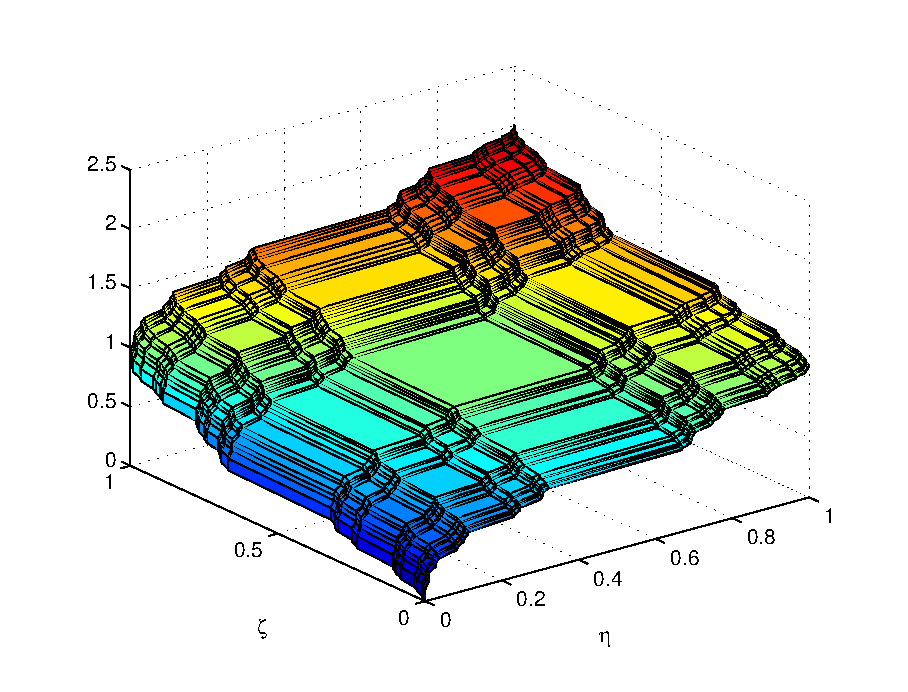
\includegraphics[width=4.38in,height=3.29in]{FDESPFDA2014revised1.eps}}
\label{fig1}
\end{figure}

\begin{center}
{\bf Figure 1. The non-differentiable solution of (\ref{eq23})
when $\alpha =\frac{\ln 2}{\ln 3}$}.
\end{center}

\vskip 2mm

\noindent
\textbf{4.2\; LFVIA-II\; \textit{for the} FP \textit{Equation Defined on Cantor Sets}}\\[2mm]

In view of (\ref{eq24}) and (\ref{eq30}), we have the following formulas with
non-differentiable terms:

\begin{equation}
\label{eq38}
\begin{array}{llllll}
\varphi _1 \left( {\zeta ,\eta } \right) \\
 \;\;=\varphi _0 \left( {\zeta ,\eta } \right)-{ }_0I_\zeta ^{\left( \alpha
\right)}\left\{ {\frac{2\zeta ^\alpha }{\Gamma \left( {1+\alpha }
\right)}\frac{\partial ^\alpha }{\partial \eta ^\alpha }\varphi _0 \left(
{\zeta ,\eta } \right)-\frac{3\zeta ^{2\alpha }}{\Gamma \left( {1+2\alpha }
\right)}\frac{\partial ^{2\alpha }}{\partial \eta ^{2\alpha }}\varphi _0
\left( {\zeta ,\eta } \right)} \right\} \\
\;\; =\frac{\eta ^\alpha }{\Gamma \left( {1+\alpha } \right)}-{ }_0I_\zeta
^{\left( \alpha \right)}\left\{ {\frac{2\zeta ^\alpha }{\Gamma \left(
{1+\alpha } \right)}\frac{\partial ^\alpha }{\partial \eta ^\alpha
}\frac{\eta ^\alpha }{\Gamma \left( {1+\alpha } \right)}-\frac{3\zeta
^{2\alpha }}{\Gamma \left( {1+2\alpha } \right)}\frac{\partial ^{2\alpha
}}{\partial \eta ^{2\alpha }}\frac{\eta ^\alpha }{\Gamma \left( {1+\alpha }
\right)}} \right\} \\
\;\; =\frac{\eta ^\alpha }{\Gamma \left( {1+\alpha } \right)}-\frac{2\zeta
^{2\alpha }}{\Gamma \left( {1+2\alpha } \right)} ,
 \end{array}
\end{equation}

\begin{equation}
\label{eq39}
\begin{array}{lllllll}
\varphi _2 \left( {\zeta ,\eta } \right) \\
\;\; =\varphi _0 \left( {\zeta ,\eta } \right)-{ }_0I_\zeta ^{\left( \alpha
\right)}\left\{ {\frac{2\zeta ^\alpha }{\Gamma \left( {1+\alpha }
\right)}\frac{\partial ^\alpha }{\partial \eta ^\alpha }\varphi _1 \left(
{\zeta ,\eta } \right)-\frac{3\zeta ^{2\alpha }}{\Gamma \left( {1+2\alpha }
\right)}\frac{\partial ^{2\alpha }}{\partial \eta ^{2\alpha }}\varphi _1
\left( {\zeta ,\eta } \right)} \right\} \\
\;\; =\frac{\eta ^\alpha }{\Gamma \left( {1+\alpha } \right)}-{ }_0I_\zeta
^{\left( \alpha \right)}\left\{ {\frac{2\zeta ^\alpha }{\Gamma \left(
{1+\alpha } \right)}\frac{\partial ^\alpha }{\partial \eta ^\alpha }\left(
{\frac{\eta ^\alpha }{\Gamma \left( {1+\alpha } \right)}-\frac{2\zeta
^\alpha }{\Gamma \left( {1+\alpha } \right)}} \right)} \right\} \\
\qquad +\;_0I_\zeta ^{\left( \alpha \right)}\left\{ {\frac{3\zeta ^{2\alpha
}}{\Gamma \left( {1+2\alpha } \right)}\frac{\partial ^{2\alpha }}{\partial
\eta ^{2\alpha }}\left( {\frac{\eta ^\alpha }{\Gamma \left( {1+\alpha }
\right)}-\frac{2\zeta ^\alpha }{\Gamma \left( {1+\alpha } \right)}} \right)}
\right\} \\
\;\; =\frac{\eta ^\alpha }{\Gamma \left( {1+\alpha } \right)}-\frac{2\zeta
^{2\alpha }}{\Gamma \left( {1+2\alpha } \right)} ,
 \end{array}
\end{equation}

\begin{equation}
\label{eq40}
\begin{array}{lllllll}
 \varphi _3 \left( {\zeta ,\eta } \right) \\
\;\; =\varphi _0 \left( {\zeta ,\eta } \right)-{ }_0I_\zeta ^{\left( \alpha
\right)}\left\{ {\frac{2\zeta ^\alpha }{\Gamma \left( {1+\alpha }
\right)}\frac{\partial ^\alpha }{\partial \eta ^\alpha }\varphi _2 \left(
{\zeta ,\eta } \right)-\frac{3\zeta ^{2\alpha }}{\Gamma \left( {1+2\alpha }
\right)}\frac{\partial ^{2\alpha }}{\partial \eta ^{2\alpha }}\varphi _2
\left( {\zeta ,\eta } \right)} \right\} \\
\;\; =\frac{\eta ^\alpha }{\Gamma \left( {1+\alpha } \right)}-{ }_0I_\zeta
^{\left( \alpha \right)}\left\{ {\frac{2\zeta ^\alpha }{\Gamma \left(
{1+\alpha } \right)}\frac{\partial ^\alpha }{\partial \eta ^\alpha }\left(
{\frac{\eta ^\alpha }{\Gamma \left( {1+\alpha } \right)}-\frac{2\zeta
^\alpha }{\Gamma \left( {1+\alpha } \right)}} \right)} \right\} \\
\qquad +\;_0I_\zeta ^{\left( \alpha \right)}\left\{ {\frac{3\zeta ^{2\alpha
}}{\Gamma \left( {1+2\alpha } \right)}\frac{\partial ^{2\alpha }}{\partial
\eta ^{2\alpha }}\left( {\frac{\eta ^\alpha }{\Gamma \left( {1+\alpha }
\right)}-\frac{2\zeta ^\alpha }{\Gamma \left( {1+\alpha } \right)}} \right)}
\right\} \\
\;\; =\frac{\eta ^\alpha }{\Gamma \left( {1+\alpha } \right)}-\frac{2\zeta
^{2\alpha }}{\Gamma \left( {1+2\alpha } \right)},
 \end{array}
\end{equation}

\begin{equation}
\label{eq41}
\begin{array}{llllll}
 \varphi _4 \left( {\zeta ,\eta } \right) \\
\;\; =\varphi _0 \left( {\zeta ,\eta } \right)-{ }_0I_\zeta ^{\left( \alpha
\right)}\left\{ {\frac{2\zeta ^\alpha }{\Gamma \left( {1+\alpha }
\right)}\frac{\partial ^\alpha }{\partial \eta ^\alpha }\varphi _3 \left(
{\zeta ,\eta } \right)-\frac{3\zeta ^{2\alpha }}{\Gamma \left( {1+2\alpha }
\right)}\frac{\partial ^{2\alpha }}{\partial \eta ^{2\alpha }}\varphi _3
\left( {\zeta ,\eta } \right)} \right\} \\
\;\; =\frac{\eta ^\alpha }{\Gamma \left( {1+\alpha } \right)}-{ }_0I_\zeta
^{\left( \alpha \right)}\left\{ {\frac{2\zeta ^\alpha }{\Gamma \left(
{1+\alpha } \right)}\frac{\partial ^\alpha }{\partial \eta ^\alpha }\left(
{\frac{\eta ^\alpha }{\Gamma \left( {1+\alpha } \right)}-\frac{2\zeta
^\alpha }{\Gamma \left( {1+\alpha } \right)}} \right)} \right\} \\
\qquad +\;_0I_\zeta ^{\left( \alpha \right)}\left\{ {\frac{3\zeta ^{2\alpha
}}{\Gamma \left( {1+2\alpha } \right)}\frac{\partial ^{2\alpha }}{\partial
\eta ^{2\alpha }}\left( {\frac{\eta ^\alpha }{\Gamma \left( {1+\alpha }
\right)}-\frac{2\zeta ^\alpha }{\Gamma \left( {1+\alpha } \right)}} \right)}
\right\} \\
\;\; =\frac{\eta ^\alpha }{\Gamma \left( {1+\alpha } \right)}-\frac{2\zeta
^{2\alpha }}{\Gamma \left( {1+2\alpha } \right)},\\
 \end{array}
\end{equation}

\begin{center}
{\bf\large .}\\
{\bf\large .}\\
{\bf\large .}\\
\end{center}

\begin{equation}
\label{eq42}
\begin{array}{llllll}
 \varphi _n \left( {\zeta ,\eta } \right) \\
\;\; =\varphi _0 \left( {\zeta ,\eta } \right)-{ }_0I_\zeta ^{\left( \alpha
\right)}\left\{ {\frac{2\zeta ^\alpha }{\Gamma \left( {1+\alpha }
\right)}\frac{\partial ^\alpha }{\partial \eta ^\alpha }\varphi _{n-1}
\left( {\zeta ,\eta } \right)-\frac{3\zeta ^{2\alpha }}{\Gamma \left(
{1+2\alpha } \right)}\frac{\partial ^{2\alpha }}{\partial \eta ^{2\alpha
}}\varphi _{n-1} \left( {\zeta ,\eta } \right)} \right\} \\
\;\; =\frac{\eta ^\alpha }{\Gamma \left( {1+\alpha } \right)}-{ }_0I_\zeta
^{\left( \alpha \right)}\left\{ {\frac{2\zeta ^\alpha }{\Gamma \left(
{1+\alpha } \right)}\frac{\partial ^\alpha }{\partial \eta ^\alpha }\left(
{\frac{\eta ^\alpha }{\Gamma \left( {1+\alpha } \right)}-\frac{2\zeta
^\alpha }{\Gamma \left( {1+\alpha } \right)}} \right)} \right\} \\
\qquad +\;_0I_\zeta ^{\left( \alpha \right)}\left\{ {\frac{3\zeta ^{2\alpha
}}{\Gamma \left( {1+2\alpha } \right)}\frac{\partial ^{2\alpha }}{\partial
\eta ^{2\alpha }}\left( {\frac{\eta ^\alpha }{\Gamma \left( {1+\alpha }
\right)}-\frac{2\zeta ^\alpha }{\Gamma \left( {1+\alpha } \right)}} \right)}
\right\} \\
\;\; =\frac{\eta ^\alpha }{\Gamma \left( {1+\alpha } \right)}-\frac{2\zeta
^{2\alpha }}{\Gamma \left( {1+2\alpha } \right)}.
 \end{array}
\end{equation}
Therefore, the non-differentiable solution of (\ref{eq23}) using (\ref{eq31}) is reported
to be as given below:

\begin{equation}
\label{eq43}
\varphi \left( {\zeta ,\eta } \right)=\mathop {\lim }\limits_{n\to \infty }
\varphi _n \left( {\zeta ,\eta } \right)=\frac{\eta ^\alpha }{\Gamma \left(
{1+\alpha } \right)}-\frac{2\zeta ^{2\alpha }}{\Gamma \left( {1+2\alpha }
\right)},
\end{equation}
which matches with the result from the LFVIA-I in Subsection 4.1.\\

\newpage

\noindent
\textbf{4.3 \; LFVIA-III \; \textit{for the} FP \textit{Equation Defined on Cantor Sets}}\\

In connection with (\ref{eq24}) and (\ref{eq31}), we set up the following formulas in the non-differentiable
forms:

\begin{equation}
\label{eq44}
\begin{array}{llllll}
 \varphi _1 \left( {\zeta ,\eta } \right) \\
\;\; =\varphi _0 \left( {\zeta ,\eta } \right)-{ }_{_0 }I_\zeta ^{\left( \alpha
\right)}\left\{ {\frac{2\zeta ^\alpha }{\Gamma \left( {1+\alpha }
\right)}\frac{\partial ^\alpha }{\partial \eta ^\alpha }\varphi _0 \left(
{\zeta ,\eta } \right)-\frac{3\zeta ^{2\alpha }}{\Gamma \left( {1+2\alpha }
\right)}\frac{\partial ^{2\alpha }}{\partial \eta ^{2\alpha }}\varphi _0
\left( {\zeta ,\eta } \right)} \right\} \\
\;\; =\frac{\eta ^\alpha }{\Gamma \left( {1+\alpha } \right)}-{ }_{_0 }I_\zeta
^{\left( \alpha \right)}\left\{ {\frac{2\zeta ^\alpha }{\Gamma \left(
{1+\alpha } \right)}\frac{\partial ^\alpha }{\partial \eta ^\alpha
}\frac{\eta ^\alpha }{\Gamma \left( {1+\alpha } \right)}-\frac{3\zeta
^{2\alpha }}{\Gamma \left( {1+2\alpha } \right)}\frac{\partial ^{2\alpha
}}{\partial \eta ^{2\alpha }}\frac{\eta ^\alpha }{\Gamma \left( {1+\alpha }
\right)}} \right\} \\
\;\; =\frac{\eta ^\alpha }{\Gamma \left( {1+\alpha } \right)}-\frac{2\zeta
^{2\alpha }}{\Gamma \left( {1+2\alpha } \right)} ,
 \end{array}
\end{equation}

\begin{equation}
\label{eq45}
\begin{array}{llllll}
 \varphi _2 \left( {\zeta ,\eta } \right)\\
\;\;=\varphi _1 \left( {\zeta ,\eta }
\right)-\;_0I_\zeta ^{\left( \alpha \right)}\left\{ {\frac{2\zeta
^\alpha }{\Gamma \left( {1+\alpha } \right)}\frac{\partial ^\alpha
}{\partial \eta ^\alpha }\varphi _1 \left( {\zeta ,\eta }
\right)-\frac{3\zeta ^{2\alpha }}{\Gamma \left( {1+2\alpha }
\right)}\frac{\partial ^{2\alpha }}{\partial \eta ^{2\alpha }}\varphi _1
\left( {\zeta ,\eta } \right)} \right\} \\
\qquad +\;_0I_\zeta ^{\left( \alpha \right)}\left\{ {\frac{2\zeta ^\alpha
}{\Gamma \left( {1+\alpha } \right)}\frac{\partial ^\alpha }{\partial \eta
^\alpha }\varphi _0 \left( {\zeta ,\eta } \right)-\frac{3\zeta ^{2\alpha
}}{\Gamma \left( {1+2\alpha } \right)}\frac{\partial ^{2\alpha }}{\partial
\eta ^{2\alpha }}\varphi _0 \left( {\zeta ,\eta } \right)} \right\} \\
\;\; =\frac{\eta ^\alpha }{\Gamma \left( {1+\alpha } \right)}-\frac{2\zeta
^\alpha }{\Gamma \left( {1+\alpha } \right)} \\
\qquad -\;_0I_\zeta ^{\left( \alpha \right)}\left\{ {\frac{2\zeta ^\alpha
}{\Gamma \left( {1+\alpha } \right)}\frac{\partial ^\alpha }{\partial \eta
^\alpha }\left( {\frac{\eta ^\alpha }{\Gamma \left( {1+\alpha }
\right)}-\frac{2\zeta ^\alpha }{\Gamma \left( {1+\alpha } \right)}}
\right)-\frac{3\zeta ^{2\alpha }}{\Gamma \left( {1+2\alpha }
\right)}\frac{\partial ^{2\alpha }}{\partial \eta ^{2\alpha }}\left(
{\frac{\eta ^\alpha }{\Gamma \left( {1+\alpha } \right)}-\frac{2\zeta
^\alpha }{\Gamma \left( {1+\alpha } \right)}} \right)} \right\} \\
\qquad  +\;_0I_\zeta ^{\left( \alpha \right)}\left\{ {\frac{2\zeta ^\alpha
}{\Gamma \left( {1+\alpha } \right)}\frac{\partial ^\alpha }{\partial \eta
^\alpha }\frac{\eta ^\alpha }{\Gamma \left( {1+\alpha }
\right)}-\frac{3\zeta ^{2\alpha }}{\Gamma \left( {1+2\alpha }
\right)}\frac{\partial ^{2\alpha }}{\partial \eta ^{2\alpha }}\frac{\eta
^\alpha }{\Gamma \left( {1+\alpha } \right)}} \right\} \\
\;\; =\frac{\eta ^\alpha }{\Gamma \left( {1+\alpha } \right)}-\frac{2\zeta
^{2\alpha }}{\Gamma \left( {1+2\alpha } \right)},
 \end{array}
\end{equation}

\begin{equation}
\label{eq46}
\begin{array}{llllll}
 \varphi _3 \left( {\zeta ,\eta } \right) \\
\;\; =\varphi _2 \left( {\zeta ,\eta } \right)-\;_0I_\zeta ^{\left( \alpha
\right)}\left\{ {\frac{2\zeta ^\alpha }{\Gamma \left( {1+\alpha }
\right)}\frac{\partial ^\alpha }{\partial \eta ^\alpha }\varphi _2 \left(
{\zeta ,\eta } \right)-\frac{3\zeta ^{2\alpha }}{\Gamma \left( {1+2\alpha }
\right)}\frac{\partial ^{2\alpha }}{\partial \eta ^{2\alpha }}\varphi _2
\left( {\zeta ,\eta } \right)} \right\} \\
\qquad +\;_0I_\zeta ^{\left( \alpha \right)}\left\{ {\frac{2\zeta ^\alpha
}{\Gamma \left( {1+\alpha } \right)}\frac{\partial ^\alpha }{\partial \eta
^\alpha }\varphi _1 \left( {\zeta ,\eta } \right)-\frac{3\zeta ^{2\alpha
}}{\Gamma \left( {1+2\alpha } \right)}\frac{\partial ^{2\alpha }}{\partial
\eta ^{2\alpha }}\varphi _1 \left( {\zeta ,\eta } \right)} \right\} \\
\;\; =\frac{\eta ^\alpha }{\Gamma \left( {1+\alpha } \right)}-\frac{2\zeta
^\alpha }{\Gamma \left( {1+\alpha } \right)} \\
\qquad -\;_0I_\zeta ^{\left( \alpha \right)}\left\{ {\frac{2\zeta ^\alpha
}{\Gamma \left( {1+\alpha } \right)}\frac{\partial ^\alpha }{\partial \eta
^\alpha }\left( {\frac{\eta ^\alpha }{\Gamma \left( {1+\alpha }
\right)}-\frac{2\zeta ^\alpha }{\Gamma \left( {1+\alpha } \right)}}
\right)-\frac{3\zeta ^{2\alpha }}{\Gamma \left( {1+2\alpha }
\right)}\frac{\partial ^{2\alpha }}{\partial \eta ^{2\alpha }}\left(
{\frac{\eta ^\alpha }{\Gamma \left( {1+\alpha } \right)}-\frac{2\zeta
^\alpha }{\Gamma \left( {1+\alpha } \right)}} \right)} \right\} \\
\qquad +\;_0I_\zeta ^{\left( \alpha \right)}\left\{ {\frac{2\zeta ^\alpha
}{\Gamma \left( {1+\alpha } \right)}\frac{\partial ^\alpha }{\partial \eta
^\alpha }\left( {\frac{\eta ^\alpha }{\Gamma \left( {1+\alpha }
\right)}-\frac{2\zeta ^\alpha }{\Gamma \left( {1+\alpha } \right)}}
\right)-\frac{3\zeta ^{2\alpha }}{\Gamma \left( {1+2\alpha }
\right)}\frac{\partial ^{2\alpha }}{\partial \eta ^{2\alpha }}\left(
{\frac{\eta ^\alpha }{\Gamma \left( {1+\alpha } \right)}-\frac{2\zeta
^\alpha }{\Gamma \left( {1+\alpha } \right)}} \right)} \right\} \\
\;\; =\frac{\eta ^\alpha }{\Gamma \left( {1+\alpha } \right)}-\frac{2\zeta
^{2\alpha }}{\Gamma \left( {1+2\alpha } \right)},
 \end{array}
\end{equation}

\begin{equation}
\label{eq47}
\begin{array}{lllllll}
 \varphi _4 \left( {\zeta ,\eta } \right) \\
\;\; =\varphi _3 \left( {\zeta ,\eta } \right)-\; _0I_\zeta ^{\left( \alpha
\right)}\left\{ {\frac{2\zeta ^\alpha }{\Gamma \left( {1+\alpha }
\right)}\frac{\partial ^\alpha }{\partial \eta ^\alpha }\varphi _3 \left(
{\zeta ,\eta } \right)-\frac{3\zeta ^{2\alpha }}{\Gamma \left( {1+2\alpha }
\right)}\frac{\partial ^{2\alpha }}{\partial \eta ^{2\alpha }}\varphi _3
\left( {\zeta ,\eta } \right)} \right\} \\
\qquad+\;_{_0 }I_\zeta ^{\left( \alpha \right)}\left\{ {\frac{2\zeta ^\alpha
}{\Gamma \left( {1+\alpha } \right)}\frac{\partial ^\alpha }{\partial \eta
^\alpha }\varphi _2 \left( {\zeta ,\eta } \right)-\frac{3\zeta ^{2\alpha
}}{\Gamma \left( {1+2\alpha } \right)}\frac{\partial ^{2\alpha }}{\partial
\eta ^{2\alpha }}\varphi _2 \left( {\zeta ,\eta } \right)} \right\} \\
\;\; =\frac{\eta ^\alpha }{\Gamma \left( {1+\alpha } \right)}-\frac{2\zeta
^\alpha }{\Gamma \left( {1+\alpha } \right)} \\
\qquad +\; _0I_\zeta ^{\left( \alpha \right)}\left\{ {\frac{2\zeta ^\alpha
}{\Gamma \left( {1+\alpha } \right)}\frac{\partial ^\alpha }{\partial \eta
^\alpha }\left( {\frac{\eta ^\alpha }{\Gamma \left( {1+\alpha }
\right)}-\frac{2\zeta ^\alpha }{\Gamma \left( {1+\alpha } \right)}}
\right)-\frac{3\zeta ^{2\alpha }}{\Gamma \left( {1+2\alpha }
\right)}\frac{\partial ^{2\alpha }}{\partial \eta ^{2\alpha }}\left(
{\frac{\eta ^\alpha }{\Gamma \left( {1+\alpha } \right)}-\frac{2\zeta
^\alpha }{\Gamma \left( {1+\alpha } \right)}} \right)} \right\} \\
\qquad -\;_0I_\zeta ^{\left( \alpha \right)}\left\{ {\frac{2\zeta ^\alpha
}{\Gamma \left( {1+\alpha } \right)}\frac{\partial ^\alpha }{\partial \eta
^\alpha }\left( {\frac{\eta ^\alpha }{\Gamma \left( {1+\alpha }
\right)}-\frac{2\zeta ^\alpha }{\Gamma \left( {1+\alpha } \right)}}
\right)-\frac{3\zeta ^{2\alpha }}{\Gamma \left( {1+2\alpha }
\right)}\frac{\partial ^{2\alpha }}{\partial \eta ^{2\alpha }}\left(
{\frac{\eta ^\alpha }{\Gamma \left( {1+\alpha } \right)}-\frac{2\zeta
^\alpha }{\Gamma \left( {1+\alpha } \right)}} \right)} \right\} \\
\;\; =\frac{\eta ^\alpha }{\Gamma \left( {1+\alpha } \right)}-\frac{2\zeta
^{2\alpha }}{\Gamma \left( {1+2\alpha } \right)} ,\\
\end{array}
\end{equation}

\begin{center}
{\bf\large .}\\
{\bf\large .}\\
{\bf\large .}\\
\end{center}

\begin{equation}
\label{eq48}
\begin{array}{lllllll}
 \varphi _n \left( {\zeta ,\eta } \right) \\
\;\; =\varphi _{n-1} \left( {\zeta ,\eta } \right)-\;_0I_\zeta ^{\left(
\alpha \right)}\left\{ {\frac{2\zeta ^\alpha }{\Gamma \left( {1+\alpha }
\right)}\frac{\partial ^\alpha }{\partial \eta ^\alpha }\varphi _{n-1}
\left( {\zeta ,\eta } \right)-\frac{3\zeta ^{2\alpha }}{\Gamma \left(
{1+2\alpha } \right)}\frac{\partial ^{2\alpha }}{\partial \eta ^{2\alpha
}}\varphi _{n-1} \left( {\zeta ,\eta } \right)} \right\} \\
\qquad +\;_0I_\zeta ^{\left( \alpha \right)}\left\{ {\frac{2\zeta ^\alpha
}{\Gamma \left( {1+\alpha } \right)}\frac{\partial ^\alpha }{\partial \eta
^\alpha }\varphi _{n-2} \left( {\zeta ,\eta } \right)-\frac{3\zeta ^{2\alpha
}}{\Gamma \left( {1+2\alpha } \right)}\frac{\partial ^{2\alpha }}{\partial
\eta ^{2\alpha }}\varphi _{n-2} \left( {\zeta ,\eta } \right)} \right\} \\
\;\; =\frac{\eta ^\alpha }{\Gamma \left( {1+\alpha } \right)}-\frac{2\zeta
^\alpha }{\Gamma \left( {1+\alpha } \right)} \\
\qquad +\;_0I_\zeta ^{\left( \alpha \right)}\left\{ {\frac{2\zeta ^\alpha
}{\Gamma \left( {1+\alpha } \right)}\frac{\partial ^\alpha }{\partial \eta
^\alpha }\left( {\frac{\eta ^\alpha }{\Gamma \left( {1+\alpha }
\right)}-\frac{2\zeta ^\alpha }{\Gamma \left( {1+\alpha } \right)}}
\right)-\frac{3\zeta ^{2\alpha }}{\Gamma \left( {1+2\alpha }
\right)}\frac{\partial ^{2\alpha }}{\partial \eta ^{2\alpha }}\left(
{\frac{\eta ^\alpha }{\Gamma \left( {1+\alpha } \right)}-\frac{2\zeta
^\alpha }{\Gamma \left( {1+\alpha } \right)}} \right)} \right\} \\
\qquad -\;_0I_\zeta ^{\left( \alpha \right)}\left\{ {\frac{2\zeta ^\alpha
}{\Gamma \left( {1+\alpha } \right)}\frac{\partial ^\alpha }{\partial \eta
^\alpha }\left( {\frac{\eta ^\alpha }{\Gamma \left( {1+\alpha }
\right)}-\frac{2\zeta ^\alpha }{\Gamma \left( {1+\alpha } \right)}}
\right)-\frac{3\zeta ^{2\alpha }}{\Gamma \left( {1+2\alpha }
\right)}\frac{\partial ^{2\alpha }}{\partial \eta ^{2\alpha }}\left(
{\frac{\eta ^\alpha }{\Gamma \left( {1+\alpha } \right)}-\frac{2\zeta
^\alpha }{\Gamma \left( {1+\alpha } \right)}} \right)} \right\} \\
\;\; =\frac{\eta ^\alpha }{\Gamma \left( {1+\alpha } \right)}-\frac{2\zeta
^{2\alpha }}{\Gamma \left( {1+2\alpha } \right)}.
 \end{array}
\end{equation}
Therefore, the non-differentiable solution of (\ref{eq21}) using (\ref{eq26}) is also
reported to be as follows:
\begin{equation}
\label{eq49}
\varphi \left( {\zeta ,\eta } \right)=\mathop {\lim }\limits_{n\to \infty }
\varphi _n \left( {\zeta ,\eta } \right)=\frac{\eta ^\alpha }{\Gamma \left(
{1+\alpha } \right)}-\frac{2\zeta ^{2\alpha }}{\Gamma \left( {1+2\alpha }
\right)},
\end{equation}
which is in conformity with the results from the LFVIA-I and LFVIA-II
in Subsections 4.1 and 4.2, respectively.\\

\vskip 2mm

\section{\; Conclusions}

In the present work, the linear FP equation defined on Cantor sets was
solved by using the LFVIAs and its closed solution is obtained. By comparing
with the LFVIA-I and the LFVIA-III, we conclude that the case of the LFVIA-II
is the best way to obtain the non-differentiable solutions of linear local fractional
partial differential equations.

\begin{thebibliography}{99}

\bibitem{1}
A. A. Kilbas, H. M. Srivastava and J. J. Trujillo,
\textit{Theory and Applications of Fractional Differential Equations},
North-Holland Mathematical Studies,
Vol. \textbf{204}, Elsevier (North-Holland) Science
Publishers, Amsterdam, London and New York, 2006.

\bibitem{2}
B. J. West, M. Bologna and P. Grigolini, {\it Physics of Fractal Operators},
Springer, Berlin, Heidelberg and New York, 2003.

\bibitem{3}
D. Baleanu, K. Diethelm, E. Scalas and J. J. Trujillo, \textit{Fractional
Calculus$:$ Models and Numerical Methods}, Series on Complexity,
Nonlinearity and Chaos, Vol. {\bf 3}, World Scientific
Publishing Company, Singapore, New Jersey, London and Hong Kong, 2012.

\bibitem{4}
M. D. Ortigueira, \textit{Fractional Calculus for Scientists and Engineers},
Springer, Berlin, Heidelberg and New York, 2011.

\bibitem{5}
S. Hu, Y.-Q. Chen and T.-S. Qiu, {\it Fractional Processes
and Fractional-Order Signal Processing$:$
Techniques and Applications}, Springer, Berlin, Heidelberg and New York, 2012.

\bibitem{6}
R. L. Magin, {\it Fractional Calculus in Bioengineering}, Begerll House,
West Redding, Connecticut, 2006.

\bibitem{7}
F. Mainardi, \textit{Fractional Calculus and Waves in Linear Viscoelasticity$:$
An Introduction to Mathematical Models}, World Scientific Publishing Company,
Singapore, New Jersey, London and Hong Kong, 2010.

\bibitem{8}
J. Klafter, S.-C. Lim and R. Metzler, \textit{Fractional Calculus$:$ Recent
Advances}, World Scientific Publishing Company,
Singapore, New Jersey, London and Hong Kong, 2011.

\bibitem{9}
V. E. Tarasov, {\it Fractional Dynamics$:$ Applications of Fractional
Calculus to Dynamics of Particles$,$
Fields and Media}, Springer, Berlin, Heidelberg and New York, 2011.

\bibitem{10}
R. Metzler, E. Barkai and J. Klafter, Deriving fractional Fokker-Planck
equations from a generalised
master equation, {\it Europhys. Lett.} {\bf 46}, 431--436 (1999).

\bibitem{11}
R. Metzler and T. F. Nonnenmacher, Space- and
time-fractional diffusion and wave equations,
fractional Fokker-Planck equations, and physical motivation,
{\it Chem. Phys.} {\bf 284}, 67--90 (2002).

\bibitem{12}
E. Barkai, Fractional Fokker-Planck equation, solution, and application,
\textit{Phys. Rev. E} {\bf 63} (4), Article ID 046118, 1--5 (2001).

\bibitem{13}
Z. Odibat and S. Momani, Numerical solution of Fokker-Planck equation with space- and
time-fractional derivatives, \textit{Phys. Lett. A} {\bf 369} (2007), 349--358 (2007).

\bibitem{14}
W. Deng,  (2008). Finite element method for the space
and time fractional Fokker-Planck equation,
{\it SIAM J. Numer. Anal.} {\bf 47}, 204--226 (2008).

\bibitem{15}
G. Jumarie,  A Fokker-Planck equation of fractional order with respect to time,
{\it J. Math. Phys.} {\bf 33}, 3536--3542 (1992).

\bibitem{16}
S. A. El-Wakil and M. A. Zahran, Fractional Fokker-Planck equation, {\it Chaos
Soliton. Fract.} {\bf 11}, 791--798 (2000).

\bibitem{17}
V. E. Tarasov, Fokker-Planck equation for fractional systems,
{\it Int. J. Mod. Phys. B} {\bf 21}, 955--967 (2007).

\bibitem{18}
V. E. Tarasov, Fractional Fokker-Planck equation for fractal media,
{\it Chaos} {\bf 15} (2), Article ID 023102, 1--8 (2005).

\bibitem{19}
D. A. Benson, S. W. Wheatcraft and M. M. Meerschaert, The fractional order
governing equation of L\'{e}vy motion, {\it Water Resour. Res.}
{\bf 36}, 1413--1423 (2000).

\bibitem{20}
F. Liu, V. Anh and I. Turner, Numerical solution of
the space fractional Fokker-Planck equation,
{\it J. Comput. Appl. Math.} {\bf 166}, 209--219 (2004).

\bibitem{21}
S. Chen, F. Liu, P. Zhuang and V. Anh, Finite difference approximations for the
fractional Fokker-Planck equation. {\it Appl. Math. Mod.} {\bf 33}, 256--273 (2009).

\bibitem{22}
X.-J. Yang, {\it Local Fractional Functional Analysis and Its Applications},
Asian Academic Publisher Limited, Hong Kong, 2011.

\bibitem{23}
X.-J. Yang, {\it Advanced Local Fractional Calculus and Its Applications},
World Science Publisher, New York, 2012.

\bibitem{24}
K. M. Kolwankar and A. D. Gangal, Local fractional Fokker-Planck equation,
{\it Phys. Rev. Lett.} {\bf 80}, 214--217 (1998).

\bibitem{25}
A. Carpinteri, B. Chiaia and P. Cornetti, On the mechanics of quasi-brittle materials
with a fractal microstructure, {\it Eng. Fract. Mech.} {\bf 70}, 2321--2349 (2003).

\bibitem{26}
F. Ben Adda and J. Cresson, About non-differentiable functions,
{\it J. Math. Anal. Appl.} {\bf 263}, 721--737 (2001).

\bibitem{27}
A. Babakhani and V. Daftardar-Gejji, On calculus of local fractional derivatives,
{\it J. Math. Anal. Appl.} {\bf 270}, 66--79 (2002).

\bibitem{28}
Y. Chen, Y. Yan and K. Zhang, On the local fractional derivative,
{\it J. Math. Anal. Appl.} {\bf 362}, 17--33 (2010).

\bibitem{29}
W. Chen, H. Sun, X. Zhang and D. Koro\v{s}ak, Anomalous diffusion modeling by
fractal and fractional derivatives, {\it Comput. Math.
Appl.} {\bf 59}, 1754--1758 (2010).

\bibitem{30}
X.-J. Yang, H. M. Srivastava, J.-H. He and D. Baleanu,
Cantor-type cylindrical-coordinate method for differential equations
with local fractional derivatives, {\it Phys. Lett. A}
{\bf 377}, 1696--1700 (2013).

\bibitem{31}
H. M. Srivastava, A. K. Golmankhaneh, D. Baleanu and X.-J. Yang,
Local fractional Sumudu transform with application to IVPs on Cantor sets,
{\it Abstr. Appl. Anal.} {\bf 2014}, Article ID 620529, 1--7 (2014).

\bibitem{32}
A.-M. Yang, J. Lie, H. M. Srivastava, G.-N. Xie and X.-J. Yang,
Local fractional Laplace variational iteration method for solving
linear partial differential equations with local fractional derivative,
{\it Discr, Dyn. Nat. Soc.} {\bf 2014}, Article ID 365981, 1--8 (2014).

\bibitem{33}
J.-H. He, A tutorial review on
fractal spacetime and fractional calculus,
{\it Int. J. Theor. Phys.} {\bf 53}, 3698--3718 (2014).

\bibitem{34}
B. B. Mandelbrot, {\it The Fractal Geometry of Nature},
W. H. Freeman and Company, New York, 1977.

\bibitem{35}
X.-J. Yang and D. Baleanu, Fractal heat conduction problem solved by local
fractional variation iteration method, {\it Therm. Sci.}
{\bf 17}, 625--628 (2013).

\bibitem{36}
X.-J. Yang, D. Baleanu, Y. Khan and S. T. Mohyud-Din,
Local fractional variational iteration method for
diffusion and wave equations on Cantor sets,
{\it Rom. J. Phys.} {\bf 59}, 36--48 (2014).

\bibitem{37}
X.-J. Yang and D. Baleanu, Local fractional variational iteration
method for Fokker-Planck equation on a Cantor set,
{\it Acta Univ.} {\bf 23}, 3--8 (2013).

\bibitem{38}
S.-H. Yan, X.-H. Chen, G.-N. Xie, C. Cattani and X.-J. Yang,
Solving Fokker-Planck equations on Cantor sets
using local fractional decomposition method,
{\it Abstr. Appl. Anal.} {\bf 2014}, Article ID 396469, 1--6 (2014).

\bibitem{39}
X.-J. Yang and F.-R. Zhang, Local fractional variational iteration method
and its algorithms, {\it Adv. Comput. Math. Appl.} {\bf 1}, 139--145 (2012).

\bibitem{40}
H.-Y. Liu, J.-H. He and Z.-B. Li, Fractional calculus for nanoscale
flow and heat transfer, {\it Int. J. Numer. Meth. Heat Fluid Flow}
{\bf 24}, 1227--1250 (2014).

\bibitem{41}
Y. Zhang, Solving initial-boundary value problems for local fractional differential equation
by local fractional Fourier series method, {\it Abstr. Appl. Anal.} {\bf 2014},
Article ID 912464, 1--5 (2014).

\bibitem{42}
O. Dovgoshey, O. Martio, V. Ryazanov and M. Vuorinen, The Cantor function,
{\it Expo. Math.} {\bf 24}, 1--37 (2006).

\bibitem{43}
D. Baleanu and X.-J. Yang, Euler-Lagrange equations on Cantor sets,
in {\it ASME $2013$ International Design Engineering Technical Conferences and Computers and
Information in Engineering Conference}, pp. V004T08A016--V004T08A016,
American Society of Mechanical Engineers, New York, 2013.

\bibitem{44}
X.-J. Yang, J. Hristov, H. M. Srivastava and B. Ahmad,
Modelling fractal waves on shallow water surfaces via local fractional
Korteweg-de Vries equation, {\it Abstr. Appl. Anal.} {\bf 2014},
Article ID 278672, 1-10 (2014).

\bibitem{45}
R. Gorenflo, F. Mainardi and H. M. Srivastava, Special
functions in fractional relaxation-oscillation and
fractional diffusion-wave phenomena,
\textit{Proceedings of the Eighth International Colloquium on
Differential Equations} (Plovdiv, Bulgaria; August 18-23, 1997)
(D. Bainov, Editor), VSP Publishers, Utrecht and Tokyo, pp. 195--202 (1998).

\end{thebibliography}


\emergencystretch=\hsize

\begin{center}
\rule{6 cm}{0.02 cm}
\end{center}

\end{document}








\end{document}
